% !TeX program = XeLaTeX
% !TeX root=./main.tex
% Edit by:XAjzh and 
\setlength{\abovedisplayskip}{5pt}
\setlength{\belowdisplayskip}{5pt}

\chapter{多维随机变量及其分布}\label{cha:3}
在有些随机现象中, 对每个样本点 $\omega$ 只用一个随机变量去描述是不够的, 
譬如要研究儿童的生长发育情况, 仅研究儿童的身高 $X(\omega)$ 或仅研究其体重 $Y(\omega)$都是片面的, 
有必要把 $X(\omega)$ 和 $Y(\omega)$ 作为一个整体来考虑, 讨论它们总体变化的统计规律性, 
进一步可以讨论 $X(\omega)$ 与 $Y(\omega)$ 之间的关系, 在有些随机现象中, 甚至要同时研究二个以上随机变量. 

如何来研究多维随机变量的统计规律性呢, 仿一维随机变量, 我们先研究联合分布函数, 
然后研究离散随机变量的联合分布列、连续随机变量的联合密度函数. 

\section{多维随机变量及其联合分布}\label{sec:3.1}

\subsection{多维随机变量}\label{ssec:3.1.1}
下面我们先给出 $n$ 维随机变量的定义. 
\begin{definition}{随机变量}{3.1.1}
	如果 $X_1(\omega),X_2(\omega),\ldots,X_n(\omega)$ 是定义在同一
	样本空间 $\Omega=\left\{\omega\right\}$ 上的 $n$ 个随机变量, 则称
	\[
	X(\omega)=(X_1(\omega),X_2(\omega),\ldots,X_n(\omega))
	\]
	为 $n$ 维(或 $n$ 元)\textbf{随机变量}\index{S!随机变量}或\textbf{随机向量}\index{S!随机向量}. 
\end{definition}
注意, 多维随机变量的关键是定义在同一样本空间上, 对于不同样本空间上的两个随机变量, 我们只能在
乘积空间 $\Omega_1\times \Omega_2=\left\{(\omega_1,\omega_2);\omega_1 \in \Omega_1,\omega_2 \in \Omega_2 \right\}$ 上讨论, 
 这要用到更多的工具, 本章将不涉及这类问题. 
      
 在实际问题中, 多维随机变量的情况是经常会遇到的臂如
  \begin{itemize}
  	\item 在研究四岁至六岁儿童的生长发育情况时, 我们感兴趣于每个儿童(样本点 $\omega$ )的身高 $X_1(\omega)$ 
  	和体重 $X_2(\omega)$ . 这里 $(X_1(\omega),X_2(\omega))$是一个二维随机变量. 
  	\item 在研究每个家庭的支出情况时, 我们感兴趣于每个家庭(样本点 $\omega$ )的衣食住行四个方面, 
  	若用 $X_1(\omega),X_2(\omega),X_3(\omega),X_4(\omega)$ 分别表示衣食住行的花费占其家庭总收人的百分比, 
  	则 $X_1(\omega),X_2(\omega),X_3(\omega),X_4(\omega)$ 就是一个四维随机变量. 
  \end{itemize}

  \subsection{联合分布函数}\label{ssec:3.1.2}
  \begin{definition}{联合分布函数}{3.1.2}
  	对任意的 $n$ 个实数 $x_1,x_2,\ldots,x_n ,$ 则 $n$ 个事件 $\{X_1\leq x_1\},\{X_2 \leq x_2\},\ldots,\{X_n\leq x_n\}$ 同时发生的概率
    \begin{equation}
    	F\left(x_{1}, x_{2}, \cdots, x_{n}\right)=P\left(X_{1} \leq x_{1}, X_{2} \leq x_{2}, \ldots, X_{n} \leq x_{n}\right)\label{eq:3.1.1}
    \end{equation}
	称为 $n$ 维随机变量 $(X_1,X_2,\ldots,X_n)$ 的\textbf{联合分布函数}\index{L!联合分布函数}. 
  \end{definition}
   本章主要研究二维随机变量, 二维以上的情况可类似进行. 

   在二维随机变量 $(X,Y)$ 场合, 联合分布函数 $F(x,y)=P(X\leq x,Y\leq y)$ 是事件 $\{X\leq x\}$ 与 $\{Y \leq y\}$ 同时发生(交)的概率. 
   如果将二维随机变量 $(X,Y)$ 看成是平面上随机点的坐标, 那么联合分布函数 $F(x,y)$ 在 $(x,y)$ 处的函数值就是随机点 $(X, Y)$ 落在
   以 $(x,y)$ 为右上角的无穷矩形内的概率, 见图~\ref{fig:3.1.1} .
   \begin{figure}[htbp]
   	\centering
   	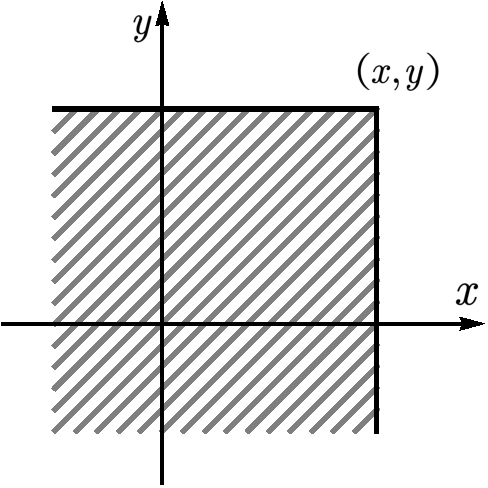
\includegraphics[width=0.4\textwidth]{fig3-1-1.pdf}
   	\caption{联合分布函数示意图}\label{fig:3.1.1}
   \end{figure}
   \begin{theorem}{}{3.1.1}
   	任一二维联合分布函数 $F(x,y)$ 必具有如下四条基本性质: 
    \begin{enumerate}
    	\item \textbf{单调性}\quad $F(x,y)$ 分别对 $x$ 或 $y$ 是单调不减的,即
    	\begin{itemize}
    		\item 当 $x_1<x_2$ 时, 有 $F(x_1,y)\leq F(x_2,y)$.
    		\item 当 $y_1<y_2$ 时, 有 $F(x,y_1)\leq F(x,y_2)$. 
    	\end{itemize}
    	\item \textbf{有界性}\quad 对任意的 $x$ 和 $y$, 有 $0\leq F(x,y) \leq 1$, 且
    	\begin{align*}
    		&F(-\infty,y)=\lim_{x\to -\infty}F(x,y)=0,	&\hspace*{3cm} \\
    		&F(x,-\infty)=\lim_{y\to -\infty}F(x,y)=0,	&\\
    		&F(+\infty,+\infty)=\lim_{x,y\to +\infty}(x,y)=1.&
    	\end{align*}
    	\item \textbf{右连续性}\quad  对每个变量都是右连续的,即
    		\begin{align*} 
    			F(x+0, y) &=F(x, y), &\hspace*{3cm} \\ 
    			F(x, y+0) &=F(x, y). &
    		\end{align*}
    	\item \textbf{非负性}\quad 对任意的 $a<b,c<d$ 有
    		\begin{equation*}
    		 	P(a<X \leq b, c<Y \leq d)= F(b, d)-F(a, d)-F(b, c)+ F(a, c) \geq 0 .
    		\end{equation*}
    \end{enumerate}
   \end{theorem}
   \begin{proof}
    	\begin{enumerate}
    		\item  因为当 $x_1<x_2$ 时, 有 $\{X_1\leq x_1\} \subset \{X_2 \leq x_2\}$, 所以对任意给定的 $y$ 有
    		\[
    			\left\{X \leq x_{1}, Y \leq y\right\} \subseteq \{ X \leq x_{2}, Y \leq y \},
    		\]
    		由此可得
    		\[
    			F\left(x_{1}, y\right)=P\left(X \leq x_{1}, Y \leq y\right) \leq 
    			P\left(X \leq x_{2}, Y \leq y\right)=F\left(x_{2}, y\right),
    		\]
    		即 $F(x,y)$ 关于 $x$ 是单调不减的, 同理可证 $F(x,y)$ 关于 $y$ 是单调不减的.
    		\item 由概率的性质可知 $0\leq F(x,y) \leq 1$. 又因为对任意的正整数 $n$ 有
    		\begin{align*}
    			&\lim_{x\to -\infty}\{X\leq x\}=\lim_{n\to +\infty}\bigcap_{m=1}^n \{X\leq -m\}=\varnothing,	\\
    			&\lim_{x\to +\infty}\{X\leq x\}=\lim_{n\to +\infty}\bigcup_{m=1}^n\{X\leq m\}=\Omega,
    		\end{align*}
    		对 $Y \leq y$ 也类似可得. 再由概率的连续性, 就可得
    		\[
    		 	F(-\infty, y)=F(x,-\infty)=0; \quad F(+\infty,+\infty)=1.
    		\]
    		\item 固定 $y$, 仿一维分布函数右连续的证明, 就可得知 $F(x, y)$ 关于 $x$ 是右连续的. 同样固定 $x$ 可
    		证得 $F(x,y)$ 关于 $y$ 是右连续的.
        	\item 只需证
        	\[
        	 	P(a<X \leq b, c<Y \leq d)=F(b, d)-F(a, d)-F(b, c)+F(a, c).
        	\]
        	为此记 ( 见图~\ref{fig:3.1.2} )
        	\[
        	 	A=\{X \leqslant a\}, \quad B=\{ X \leqslant b \}, \quad C=\{Y \leqslant c\}, \quad D=\{Y \leqslant d\},
        	\]
        	考虑到
        	\[
        	 	\{ a<X \leqslant b \}=B-A=B \cap \overline{A}, \quad\{c<Y \leqslant d\}=D-C=D \cap \overline{C},
        	\]
        	且 $A \subset B, C\subset D,$ 由此可得
        	\begin{align*}
        		 0 & \leqslant P(a<X \leqslant b, c<Y \leqslant d) \\ 
        		 &=P(B \cap \overline{A} \cap D \cap \overline{C}) \\ 
        		 &=P(B D-(A \cup C)) \\ 
        		 &=P(B D)-P(A B D \cup B C D) \\ 
        		 &=P(B D)-P(A D \cup B C) \\ 
        		 &=P(B D)-P(A D)-P(B C)+P(A B C D) \\ 
        		 &=P(B D)-P(A D)-P(B C)+P(A C ) \\ 
        		 &=P(B D)-P(A D)-P(B C)+P(A B C D) \\ 
        		 &=F(b, d)-F(a, d)-F(b, c)+F(a, c). 
        	\end{align*}
    	\end{enumerate}
    \end{proof}
   \begin{figure}[htbp]
   	\centering
   	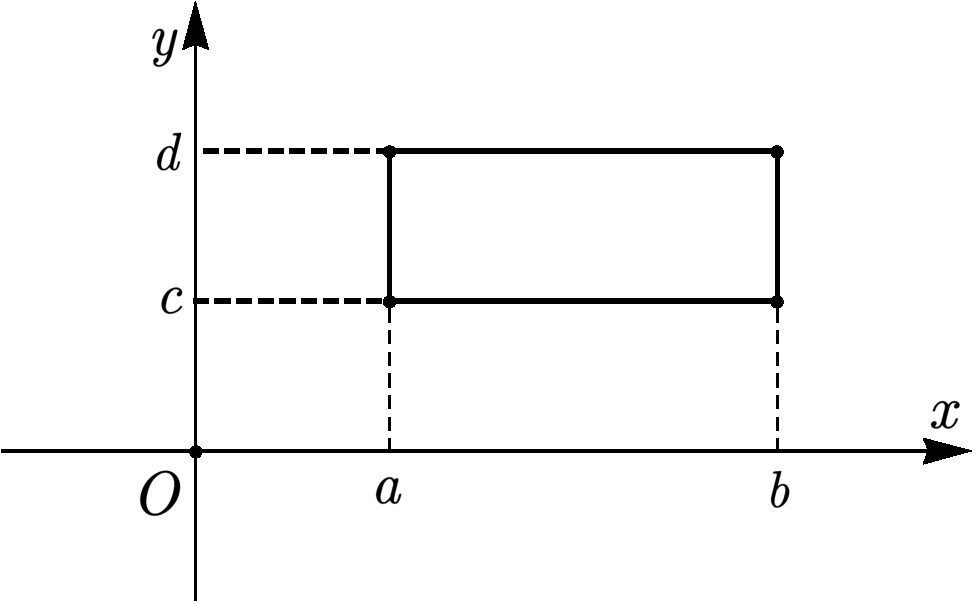
\includegraphics[width=0.4\textwidth]{fig3-1-2.pdf}
   	\caption{二维随机变量 $(X,Y)$ 落在矩形中的情况}\label{fig:3.1.2}
   \end{figure}
   还可证明,具有上述四条性质的二元函数 $F(x,y)$ 一定是某个二维随机变量的分布函数.

   任一二维分布函数 $F(x,y)$ 必具有上述四条性质, 其中性质 \textit{4} 是二维场合特有的, 也是合理的. 但性质 \textit{4} 不能
   由前三条性质推出, 必须单独列出, 且仅满足前三条性质是不够的, 因为存在这样的二元函数 $G(x,y)$ 满足
   以上性质 \textit{1,2,3}, 但它不满足性质 \textit{4}, 见下面例子.

   \begin{example}\label{exam:3.1.1}
   	二元函数
   	\[
   	 	G(x,y)=\begin{cases}
   	 		0,	& x+y<0;\\
   	 		1,	& x+y\geq 0 \\
   	 	\end{cases}
   	\]
   	满足二维分布函数的性质 \textit{1,2,3}, 但它不满足性质 \textit{4}.

    这从 $G(x,y)$ 的定义可看出: 若用 $x+y=0$ 将平面 $xOy$ 一分为二, 则
 
    $G(x,y)$ 在右上半平面 $(x+y\geq 0)$ 取值为1,
   
    $G(x,y)$ 在左下半平面 $(x+y\geq 0)$ 取值为0,

    $G(x,y)$ 具有非降性、有界性和右连续性, 但在正方形区域 $\{(x,y);-1\leq x\leq 1,-1\leq y\leq 1\}$的四个顶点上, 右上
    三个顶点位于右上半闭平面, 只有左下顶点 $(-1,-1)$ 位于左下半开平面, 故有
    \[
     	G(1,1)-G(1,-1)-G(-1,1)+G(-1,-1)=1-1-1+0=-1<0,
    \]
	所以 $G(x,y)$ 不满足性质 \textit{4}, 故 $G(x,y)$ 不能成为某二维随机变量的分布函数.
   \end{example}

   \subsection{联合分布列}\label{ssec:3.1.3}

   \begin{definition}{联合分布列}{3.1.3}
		如果二维随机变量 $(X,Y)$ 只取有限个或可列个数对 $(x_i,y_j)$, 则称 $(X,Y)$ 为二维离散随机变量, 称
    \begin{equation}\label{eq:3.1.2}
     	p_{i j}=P\left(X=x_{i}, Y=y_{j}\right), \quad i, j=1,2, \ldots
    \end{equation}
   	为 $(X,Y)$ 的\textbf{联合分布列}\index{L!联合分布列}, 也可如下用表格形式记联合分布列.
   \end{definition}
   \begin{center}
   		\begin{tabular}{cccccc}
   		\toprule
   		 & \multicolumn{5}{c}{$Y$} \\
   		 \cmidrule{2-6} 
   		 $X$	&	$y_1$&	$y_2$&	\ldots&	$y_j$& \ldots	\\
   		 \midrule 
   		 $x_1$& $p_{11}$ & $p_{12}$ & \ldots & $p_{1j}$ & \ldots \\
   		 \midrule 
   		 $x_2$& $p_{21}$ & $p_{22}$ & \ldots & $p_{2j}$ & \ldots \\
   		 \midrule 
   		 $\vdots$& $\vdots$ & $\vdots$ & $\ddots$ & $\vdots$ & $\ddots$ \\
   		 \midrule 
   		$x_i$ & $p_{i1}$ & $p_{i2}$ & \ldots & $p_{ij}$  & \ldots \\
   		\midrule 
   		 $\vdots$& $\vdots$ & $\vdots$ & $\ddots$ & $\vdots$ & $\ddots$ \\
   		 \bottomrule
   		\end{tabular} 
   \end{center}
   联合分布函数的基本性质:
   \begin{enumerate}
   	\item 非负性: $p_{ij}\geq 0$;
   	\item 正则性: $\sum_{i=1}^{+\infty}\sum_{j=1}^{+\infty}p_{ij}=1$.
   \end{enumerate}
   求二维离散随机变量的联合分布列, 关键是写出二维随机变量的可能取的数对及其发生的概率.

   \begin{example}\label{exam:3.1.2}
   		从 1,2,3,4 中任取一数记为 $X$, 再从 $1,\ldots,X$ 中任取一数记为 $Y$. 求 $(X,Y)$ 的联合分布列及 $P(X=Y)$.     
   \end{example}
   \begin{solution}
   		$(X,Y)$ 为二维离散随机变量, 其中 $X$ 的分布列为
         \[  
         	 P(X=i)=1/4,i=1,2,3,4.
         \]
		$Y$ 的可能取值也是 $1,2,3,4$, 若记 $j$ 为 $Y$ 的取值,

		 则当 $j>i$ 时,有 $P(X=i,Y=j)=P(B)=0$.
  
  		当 $1\leq j \leq i \leq 4$ 时,由乘法公式
  		\[
  		 	P(X=i, Y=j)=P(X=i) P(Y=j | X=i)=\frac{1}{4} \times \frac{1}{i}.
  		\]
		所以得 $(X,Y)$ 的联合分布列为
		\begin{center}
			\begin{tabular}{ccccc}
			\toprule
			 & \multicolumn{4}{c}{$Y$} 		 \\ 
			 \cmidrule{2-5}
			 $X$&  	1	&  2	&  3&  		4\\ 
			 \midrule
			 1 	&  1/4	&  0	&  0&  		0\\
			 \midrule
			 2	&  1/8	& 1/8 	&  0&  		0\\ 
			 \midrule
			 3	& 1/12	&  1/12	&  1/12&	0\\ 
			 \midrule
			 4&  1/16	&  1/16	&  1/16&  1/16\\ 
			 \bottomrule
			\end{tabular} 
		\end{center}
		由此可算得事件 $\{X=Y\}$ 的概率为
		\[
		 	P(X=Y)=p_{11}+p_{22}+p_{33}+p_{44}=\frac{1}{4}+\frac{1}{8}+\frac{1}{12}+\frac{1}{12}=\frac{25}{48}=0.5208
		\]
   \end{solution}
   \subsection{联合密度函数}\label{ssec:3.1.4}
   \begin{definition}{联合密度函数}{3.1.4}
   	如果存在二元非负函数 $p(x,y)$, 使得二维随机变量 $(X,Y)$ 的分布函数 $F(x,y)$ 可表示为
   	\begin{equation}\label{eq:3.1.3}
   	 	F(x, y)=\int_{-\infty}^{x} \int_{-\infty}^{y} p(u, v) \dd v \dd u
   	\end{equation}
   	则称 $(X,Y)$ 为二维连续随机变量, 称 $p(u,v)$ 为 $(X,Y)$ 的\textbf{联合密度函数}\index{L!联合密度函数}.
   \end{definition}
   在 $F(x,y)$ 偏导数存在的点上有
   \[
    	p(x, y)=\frac{\partial^{2}}{\partial x \partial y} F(x, y).
   \]
   \textbf{联合密度函数的基本性质}:
   \begin{enumerate}
   	\item \textbf{非负性}: $p(u,v)\geq 0$ 
   	\item \textbf{正则性}: $\int_{-\infty}^{+\infty} \int_{-\infty}^{+\infty} p(u, v) \dd v \dd u=1$
   \end{enumerate}
   给出联合密度函数 $p(x,y)$, 就可以求有关事件的概率了. 若 $G$ 为平面上的一个区域, 
   则事件 $\{(X,Y) \in G\}$ 的概率可表示为在 $G$ 上对 $p(x,y)$的二重积分:
   \begin{equation}\label{eq:3.1.4}
    	P((X, Y) \in G)=\iint_{G} p(x, y) \dd x \dd y.
   \end{equation}
   在具体使用上式时, 要注意积分范围是 $p(x,y)$ 的非零区域与 $G$ 的交集部分, 然后设法化成累次积分, 最后计算出结果.
   \begin{example}\label{exam:3.1.3}
   		设 $(X,Y)$ 联合密度函数为
   		\[
   		p(x, y)=\left\{
   		\begin{array}{cc}
   		6 \ee^{-2 x-3 y}, & x>0, y>0; \\
   		0, & others.
   		\end{array}\right.
   		\]
   		试求: $(1)\; P(X<1,Y>1); \; (2)\; P(X>Y)$.
   \end{example}
   \begin{solution}
  		\begin{enumerate}
  		\item 积分区域见图~中的阴影部分, 
  		\begin{align*} 
  		 P(X<1, Y>1) &=\int_{1}^{+\infty} \int_{0}^{1} 6 \ee^{-2 x-3 y} \dd x \dd y \\
  		 &=6 \int_{0}^{1} \ee^{-2 x} \dd x \int_{1}^{+\infty} \ee^{-3 x} \dd y \\ 
  		 &=\left(1-\ee^{-2}\right) \ee^{-3}=0.0430. 
  		\end{align*}
  		\item 积分区域见图3.1.3(b)中的阴影部分, 从而容易写出累次积分.
  		\begin{align*} 
  		 P(X>Y) &=\int_{0}^{+\infty} \int_{0}^{x} 6 \ee^{-2 x} \ee^{-3 y} \dd y \dd x=
  		 \int_{0}^{+\infty} 2 \ee^{-2 x}\left(1-\ee^{-3 x}\right) \dd x \\ 
  		 &=\left[-\ee^{-2 x}+\frac{1}{5} \ee^{-5 x}\right]_{0}^{+\infty}=1-\frac{1}{5}=\frac{4}{5} .
  		\end{align*}
  		\end{enumerate}             
   \end{solution}
   \begin{figure}[htbp]
   \centering
   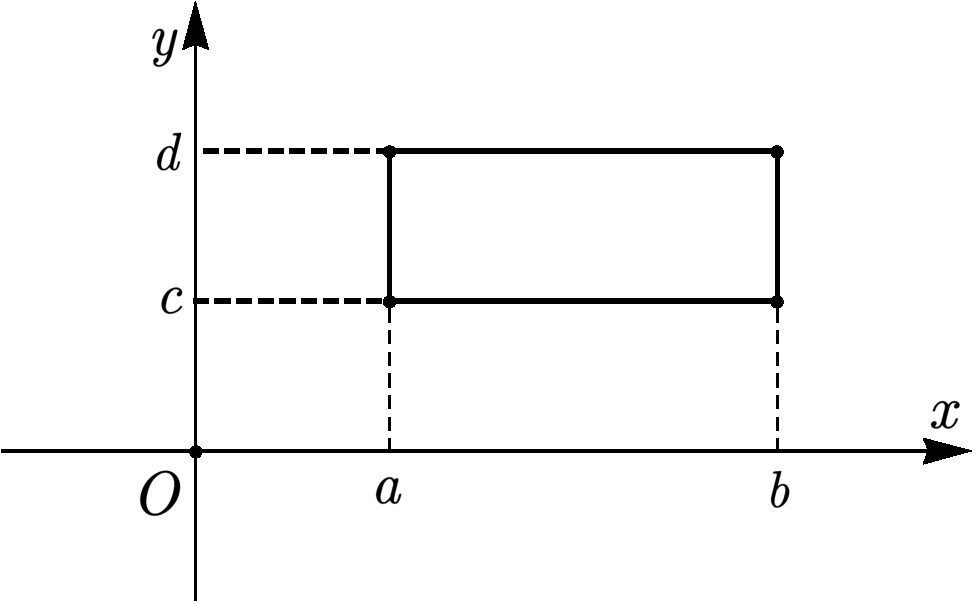
\includegraphics[width=0.4\textheight]{fig3-1-2.pdf}
   \caption{$p(x,y)$ 的非零区域与有关事件的交集部分}\label{fig:3.1.3}
   \end{figure}
   
  \subsection{常用多维分布}\label{ssec:3.1.5}
  下面介绍一些多维随机变量的常用分布. 
   
  \textbf{一、多项分布}
   
  多项分布是重要的多维离散分布, 它是二项分布的推广.
  
  进行 $n$ 次独立重复试验, 如果每次试验有 $r$ 个可能结果: $A_1, A_2$,\ldots,$A_r$, 且每次试验中 $A_i$ 发生的
  概率为 $p_{i}=P\left(A_{i}\right), i=1,2, \ldots, r . p_{1}+p_{2}+\cdots+p_{r}=1$.
  记 $X_i$ 为 $n$ 次独立重复试验中 $A_i$ 出现的次数, $i=1,2,\ldots,r$. 则 $(X_1,X_2,\ldots,X_r)$ 
  取值 $(n_1,n_2,\ldots,n_r)$ 的概率, 即 $A_1$ 出现 $n_1$ 次, $A_2$ 出现$n_2$ 次\ldots\ldots $A_r$ 出现 $n_r$ 次的概率为
  \begin{equation}
	  P\left(X_{1}=n_{1}, X_{2}=n_{2}, \ldots, X_{r}=n_{r}\right)=\frac{n !}{n_{1} ! n_{2} ! \cdots n_{r} !} p_{1}^{n_{1}} p_{2}^{n_{2}} \ldots p_{r}^{n_r},
  \end{equation}
  其中 $n=n_1+n_2+\cdots+n_r$.
  
  这个联合分布列称为 $r$ 项分布, 又称多项分布, 记为 $M(n,p_1,p_2,\ldots,p_r)$. 这个概率
  是多项式 $(p_1+p_2+\cdots+p_r)^n$ 展开式中的一项, 故其和为 1. 当 $r=2$ 时, 即为二项分布.
  \begin{example}\label{exam:3.1.4}
    一批产品共有 100 件, 其中一等品 60 件、二等品 30 件、三等品 10 件. 
    从这批产品中有放回地任取3件, 以 $X$ 和 $Y$ 分别表示取出的 3 件产品中一等品、二等品的件数, 求二维随机变量 $(X,Y)$ 的联合分布列.
  \end{example}
  \begin{solution}
    因为 $X$ 和 $Y$ 的可能取值都是 0,1,2,3, 所以记 $(X,Y)$ 的联合分布列为
    \begin{center}
      \begin{tabular}{ccccc}
        \toprule
          & \multicolumn{4}{c}{$Y$} \\
        \cmidrule{2-5}
        $X$ & 0&  1&  2&  3 \\
        \midrule
        0&  $p_{00}$& $p_{01}$& $p_{02}$& $p_{03}$\\
        \midrule
        1&  $p_{10}$& $p_{11}$& $p_{12}$& $p_{13}$\\
        \midrule
        2&  $p_{20}$& $p_{21}$& $p_{22}$& $p_{23}$\\
        \midrule
        3&  $p_{30}$& $p_{31}$& $p_{32}$& $p_{33}$\\
        \bottomrule
      \end{tabular}
    \end{center}
    当 $i+j>3$ 时, 有 $p_{ij}=0$, 即
    \[
      p_{13}=p_{22}=p_{23}=p_{31}=p_{32}=p_{33}=0.
    \]
    而当 $i+j\leq 3$ 时, 事件 $\{X=i,Y=j\}$ 表示: 取出的 3 件产品中有 $i$ 件一等品、$j$ 件二等品、$3-i-j$ 件三等品的件数, 
    所以有放回地抽取时, 对 $i+j\leq 3$, 有
    \[
      p_{i j}=\frac{3 !}{i ! j !(3-i-j) !}\left(\frac{6}{10}\right)^{i}\left(\frac{3}{10}\right)^{j}\left(\frac{1}{10}\right)^{3-i-j}.
    \]
    由以上公式, 就可具体算出 $(X,Y)$ 的联合分布列为
    \begin{center}
      \begin{tabular}{ccccc}
        \toprule
          & \multicolumn{4}{c}{$Y$} \\
        \cmidrule{2-5}
        $X$ & 0&  1&  2&  3 \\
        \midrule
        0&  0.001   & 0.009   & 0.027   & 0.027   \\
        \midrule
        1&  0.018   & 0.108   & 0.162   & 0       \\
        \midrule
        2&  0.108   & 0.324   & 0       & 0       \\
        \midrule
        3&  0.216   & 0       & 0       & 0       \\
        \bottomrule
      \end{tabular}
    \end{center}
  \end{solution}
  有此联合分布列, 就可计算有关事件的概率, 譬如
  \begin{align*}
    P(X \leq 1, Y \leq 1)&=0.001+0.009+0.018+0.108=0.136. \\
    P(X=0)=\sum_{j=0}^{3} P(X&=0, Y=j)=0.001+0.009+0.027+0.027=0.064.
  \end{align*}
  %此例是第二章~\ref{sec:2.4} 节中的二项分布的推广, 差别在于:~\ref{sec:2.4} 节中讨论的是从 " 合格品 "、" 不合格品" 两种情况中抽取, 而在
  %此是从一等品、二等品和三等品三种情况中抽取. 这里我们称它为三项分布, 它是一种特殊的多项分布.
  此例是第二章 2.4 节中的二项分布的推广, 差别在于: 2.4 中讨论的是从 " 合格品 "、" 不合格品" 两种情况中抽取, 而在此是从一等品、二等品和
  三等品三种情况中抽取. 这里我们称它为三项分布, 它是一种特殊的多项分布.